In this section, we present our \chef prototype, along with our experience preparing two symbolic execution engines, one for Python and the other for Lua.

\begin{figure}
  \centering
  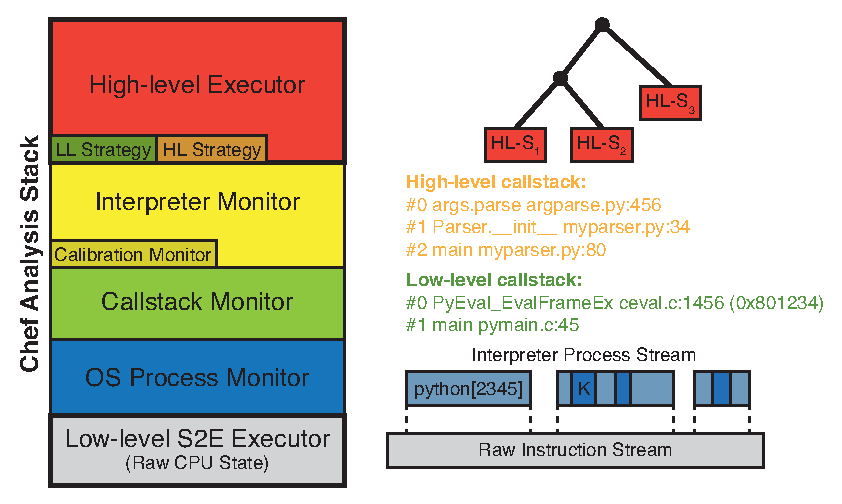
\includegraphics[width=0.7\textwidth]{evaluation/figures/chef-implem-stack}
  \caption{The implementation of \chef, as a stack of S2E analysis modules that refine the raw stream of x86 instructions into a high-level symbolic execution view.}
  \label{fig:eval:chef-implem-stack}
\end{figure}

\paragraph{Implementation}

We implemented \chef on top of the S2E analysis platform~\cite{s2eSystem}, which is a symbolic virtual machine that executes symbolically entire guests.
%
The implementation consists of a stack of dynamic analysis modules that refine the raw stream of x86 instructions at the CPU level into high-level program statements forming a symbolic execution tree (Figure~\ref{fig:eval:chef-implem-stack}).

First, the OS Monitor module breaks down the raw stream of x86 instructions into processes, and separates the user from the kernel mode.
%
The module cooperates with an instrumented Linux kernel in the VM, which reports all running threads, their creation, and termination.  To detect context switches, the OS Monitor tracks the value of the x86 CR3 page table register.  To detect user/kernel mode switches, the OS Monitor tracks the privilege level (ring) in the CPU.
%
The analysis modules above the OS Monitor look only at the user-mode instructions of the interpreter process.

Next, the Callstack Monitor tracks the \codebit{call} and \codebit{ret} instructions in the interpreter to maintain the low-level call stack.
%
On top, the Interpreter Monitor uses the low-level call stack and the interpreter HLPC slice information (Section~\ref{sec:chef:hlcf}) to maintain the high-level HLPC stack.
%
The Interpreter Monitor also computes the HLPC slice when the interpreter runs in calibration mode.

Finally, the top High-level Executor module aggregates the HLPC information from all low-level execution states to maintains the high-level symbolic execution tree.


\paragraph{Case Studies}

We used \chef to generate symbolic execution engines for Python (Section~\ref{sec:eval:python-proto}) and Lua (Section~\ref{sec:eval:lua-proto}). Table~\ref{tab:pychanges} summarizes the effort to set up the two interpreters for \chef.  The necessary changes to the interpreter amount to 274 lines of code for Python and 233 for Lua.
%
The total developer time was 5 person-days for Python and 3 person-days for Lua, which is orders of magnitude smaller than the effort required for building a complete symbolic execution engine from scratch.  

\begin{table}
\centering
\small
\begin{tabular}{|@{\hspace*{4pt}}l@{\hspace*{4pt}}|@{\hspace*{4pt}}r@{\hspace*{4pt}}|@{\hspace*{4pt}}r@{\hspace*{4pt}}|}
\hline
\textbf{Component} & \textbf{Python} & \textbf{Lua}\\
\hline
Interpreter core size (C LoC) & 427,435 & 14,553 \\
\hline
\hline
%% HLPC instrumentation (C LoC) & 47 (0.01\%) & 44 (0.30\%) \\
Symbolic optimizations (C LoC) & 274 (0.06\%) & 233 (1.58\%) \\
Native extensions (C LoC) & 1,320 (0.31\%) & 154 (1.06\%) \\
Test library (Python/Lua LoC) & 103 & 87 \\
\hline
\hline
Developer time (person-days) & 5 & 3 \\
\hline
\end{tabular}
\caption{Summary of the effort required to support Python and Lua in \chef.  The first row is the interpreter size without the standard language library. The next row shows changes in the interpreter core, while the following two constitute the symbolic test library.  The last row indicates total developer effort.}
\label{tab:pychanges}
\end{table}

\subsection{Symbolic Execution Engine for Python}
\label{sec:eval:python-proto}

\paragraph{Interpreter Preparation}

We instrumented the CPython interpreter 2.7.3 for use with \chef, according to the guidelines presented in Section~\ref{sec:chef:optimizeforsymbex}.

Python programs are composed of modules, corresponding to Python source files.  Before executing a module, the interpreter compiles its source into an interpreter-specific bytecode format, i.e., each source statement is translated into one or more lower-level primitive instructions.  The instructions are grouped into blocks, corresponding to a single loop nesting, function, method, class, or global module definition.
%
\chef automatically detects the HLPC variable pointing to the bytecode blocks, by using the HLPC slice reconstruction procedure in Section~\ref{sec:chef:hlcf}.  We cross-checked the correctness of the obtained slice by looking it up in the interpreter source code, via the debug symbols in the binary.
%% We define an \hlpc as the concatenation of the unique block address of the top frame on the stack and the current instruction offset inside the block. We instrumented the Python interpreter to pass this program location to \chef; this required adding less than 50 LoC to the main interpreter loop.

We performed several optimizations on the Python interpreter (Section~\ref{sec:chef:optimizeforsymbex}): we neutralized the hash functions of strings and integers, which are the most common objects; we concretized the memory sizes passed to the garbage-collected memory allocator; and we eliminated interning for small integers and strings.    
%
Most optimizations involved only adding preprocessor directives for conditional compilation of blocks of code.
%
We gathered the optimizations under a new \codebit{--with-symbex} flag of the interpreter's \codebit{./configure} script.

\paragraph{Symbolic Tests}

To validate the usefulness of the resulting symbolic execution engine, we use it as a test case generation tool.  To this end, we implemented a symbolic test library as a separate Python package, used both inside the guest virtual machine, and outside, during test replay.
%
Figure~\ref{fig:sample-test} is an example of a symbolic test class for the \codebit{argparse} command-line interface generator. It sets up a total of 12 symbolic characters of input: two 3-character symbolic arguments to configure the command-line parser plus another two to exercise the parsing functionality.
%
We choose three characters for each command line argument to minimally cover the three types of arguments: short option (e.g., \codebit{-h}), long option (e.g., \codebit{-{}-x}), and positional (e.g., \codebit{xyz}).

The test class derives from the library's \codebit{SymbolicTest} class, which provides two methods to be overridden: \codebit{setUp}, which is run once before the symbolic test starts, and \codebit{runTest}, which creates the symbolic input and can check properties.  The symbolic inputs are created by calling the \codebit{getString} and \codebit{getInt} methods in the \codebit{SymbolicTest} API.

\begin{figure}
  \centering
  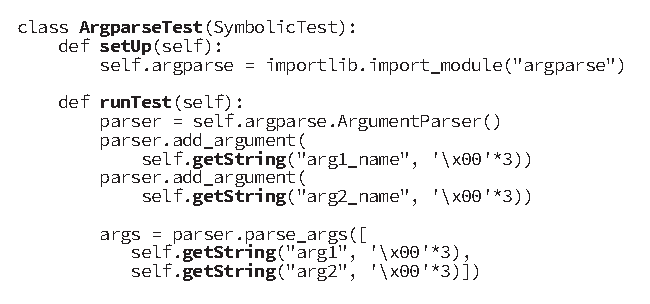
\includegraphics[width=0.7\textwidth]{evaluation/figures/symtest}
  \caption{The symbolic test used to exercise the functionality of the Python \codebit{argparse} package.}
  \label{fig:sample-test}
\end{figure}

A symbolic test is executed by a symbolic test runner, which is also part of the library.  The runner can work in either symbolic or replay mode. 
%
In \emph{symbolic mode}, the runner executes inside the guest virtual machine.  It creates a single instance of the test class, whose \codebit{getString} and \codebit{getInt} methods create corresponding Python objects and invoke the \codebit{make\_symbolic} call to mark their memory buffers as symbolic.
%
In \emph{replay mode}, the runner creates one instance of the test class for each test case created by \chef. The \codebit{getString} and \codebit{getInt} methods return the concrete input assignment of the test case.


\subsection{Symbolic Execution Engine for Lua}
\label{sec:eval:lua-proto}

Lua is a lightweight scripting language mainly used as an interpreter library to add scripting capabilities to software written in other languages. However, it also has a stand-alone interpreter and several Lua-only projects exist. We generated a symbolic execution engine for Lua based on version 5.2.2 of the Lua interpreter.

\paragraph{Interpreter Instrumentation}

Similar to Python, Lua programs are composed of one or more Lua source files, compiled into a bytecode format.  The code is compiled into a set of functions that operate on a global stack of values.  Each function is composed of a sequence of bytecode instructions, where each instruction is defined by an offset, opcode, and parameters.
%
We automatically detect updates to the HLPC variable pointing to bytecode instructions.  We cross-checked the correctness of the interpreter HLPC slice using the debug symbols in the binary.
%% We construct the \hlpc as the concatenation of the unique address of the function in the top frame and the current instruction offset being executed.  The instrumentation amounts to less than 50 LoC added to the interpreter loop.

We optimized the Lua interpreter for symbolic execution by eliminating string interning.  In addition, we configured the interpreter to use integer numbers instead of the default floating point, for which S2E does not support symbolic expressions.  This change was easy, because it was available as a macro definition in the interpreter's configuration header.

%%% Local Variables: 
%%% mode: latex
%%% eval: (visual-line-mode)
%%% fill-column: 1000000
%%% TeX-master: "main"
%%% End:
